\begin{center}
	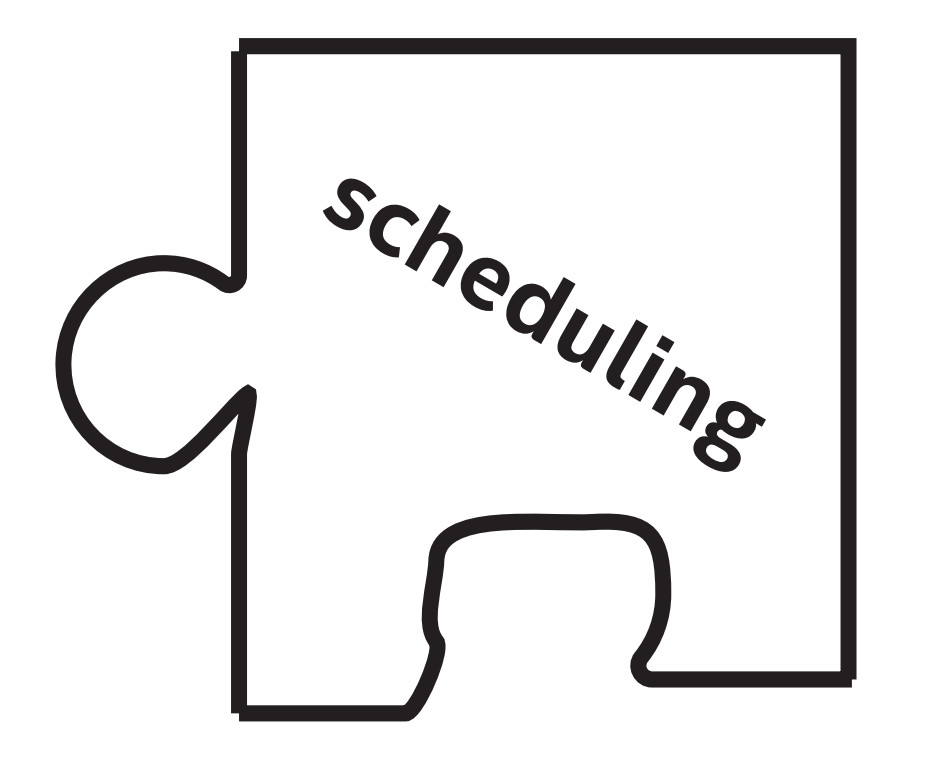
\includegraphics[width=0.3\textwidth]{content/chapter-8/images/1}
\end{center}

我们需要对并行大师进行讨论。编排并行程序是一件美妙的事情——因为把所有数据安排的明明白白,所以代码无需等待就能全速运行。并且代码进行了分解,以保持硬件最大程度的使用。\par

生活在快车道上——而不仅仅是一条车道!——我们要认真地对待调度工作。为了做到这一点,可以用任务图来规划工作。\par

本章中,我们将讨论任务图,用于正确有效地运行复杂内核序列的机制。在应用程序中,有两件事情需要排序:内核和数据移动。任务图是我们用来实现正确排序的机制。\par

首先,快速回顾如何使用依赖项来编排第3章中的任务。接下来,将介绍DPC++运行时如何构建图。我们将讨论DPC++图的基本构造块,即命令组。然后,说明构建图的不同方法。还会讨论数据移动(包括显式和隐式)如何用图表示。最后,将讨论与主机同步图的各种方法。\par